\begin{frame}
  \frametitle{Introduction and Procedure}
  \begin{columns}
        \column[t]{5cm}
        Many of the new, advanced reactors will use \gls{HALEU} fuel. 
        What are the resource requirements to meet expected \gls{HALEU}
        demand?

        \begin{block}{Procedure}
            Modeled three fuel cycle scenarios using \Cyclus. Simulations 
            model materials from mine to final disposal.
            \begin{itemize}
                \item \textbf{Scenario 1:} Current fleet of \glspl{LWR}
                \item \textbf{Scenario 2:} No growth transition to \gls{USNC} \gls{MMR}
                \item \textbf{Scenario 3:} No growth transition to X-energy Xe-100
            \end{itemize}
 
        \end{block}
        
        \column[t]{5cm}
        \begingroup
        \renewcommand{\arraystretch}{1.5} % Default value: 1
        \begin{table}[t!]
            \tiny
            \caption{Mico-reactor design specifications}
            \label{tab:reactor_summary}
            \begin{tabular}{ p{1.5cm} p{1.5cm} p{1.25cm}}
                \hline
                Design Criteria & \gls{USNC} \gls{MMR}\textsuperscript{TM} & 
                    X-Energy Xe-100\textsuperscript{TM} \\\hline
                
                Reactor Type & Modular HTGR & Modular HTGR \\
                Power Output (MWth) & 15 & 200 \\
                Enrichment (\% $^{235}U$) & 13 & 15.5 \\
                Cycle Length (years) & 20 & Online Refuel\\
                Fuel Form & TRISO Compacts & TRISO Pebbles\\
                Reactor Lifetime & 20 years & 60 years \\
                Coolant & He & He \\
                \hline
            \end{tabular}
        \end{table}   
        \endgroup
  \end{columns}
        
\end{frame}

\begin{frame}
\frametitle{Results}
        \vspace{-0.5cm}
    \begin{columns}
      \column[t]{6cm}
      \begin{figure}[t!]
          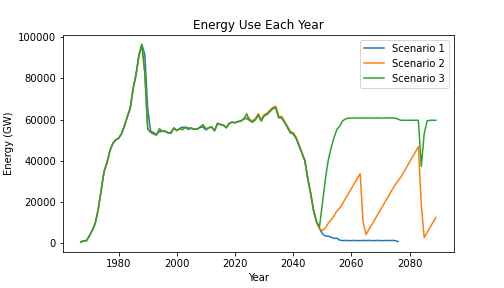
\includegraphics[trim=0 8 0 10,clip,width=\linewidth]{figures/energy_all.png}
            \vspace*{-0.5cm}
          \caption{Total energy output of each scenario.}
          \label{fig:energy}
      \end{figure}
            \vspace*{-0.25cm}
      \begin{figure}[h]
          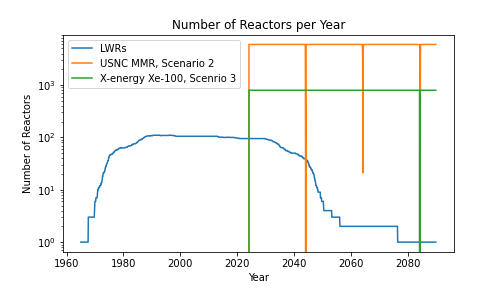
\includegraphics[trim=0 8 0 10,clip,width=\linewidth]{figures/rx_deployment_all.png}
            \vspace*{-0.5cm}
          \caption{Number of each reactor type deployed.}
          \label{fig:ex_deployment}
      \end{figure}
      \column[t]{6cm}
  \begin{figure}[t]
      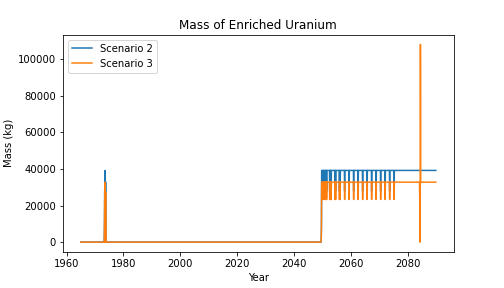
\includegraphics[trim=0 8 0 10,clip,width=\linewidth]{figures/enrichedU_advancedrx.png}
            \vspace*{-0.5cm}
      \caption{Mass of enriched uranium to supply advanced reactors.}
      \label{fig:enrichedU}
  \end{figure}
            \vspace*{-0.5cm}
  \begin{figure}[h]
      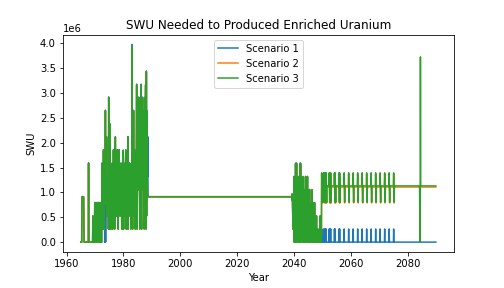
\includegraphics[trim=0 8 0 10,clip,width=\linewidth]{figures/swu_all.png}
            \vspace*{-0.5cm}
      \caption{Total \gls{SWU} capacity required to enrich natural uranium in each scenario.}
      \label{fig:swu}
  \end{figure}
  \end{columns}
\end{frame}


\begin{frame}
\frametitle{Conclusions}
    \begin{itemize}
        \item Neither of the transition scenarios (Scenarios 2 and 3) meet the desired power level.
        \item Scenario 2 requires a higher mass of \gls{HALEU} than Scenario 3.
        \item Scenario 3 requires the most \gls{SWU} capacity.
        \item Scenario 3 involves a large demand in \gls{HALEU} when 
              new reactors are built.
    \end{itemize}

    \begin{block}{Ongoing Work}
        \begin{itemize}
            \item Ensure energy demand is met by each transition scenario.
            \item Adjust feed inventory for enrichment facilities.
            \item Ensure simulations are as realistic as possible.
            \item Simulate growth transition scenarios.
            \item Include other reactor types.
        \end{itemize}
    \end{block}
    \vspace{1.7cm}
    \scriptsize
    This material is based upon work supported under an Integrated University 
Program Graduate Fellowship. Any opinions, findings, conclusions, or 
recommendations expressed in this publication are those of the author(s) 
and do not necessarily reflect the views of the Department of Energy Office 
of Nuclear Energy.

\end{frame}
